
% Section 6.1
% Testbed?

% Section 6.2
% Numerical results


To evaluate our platform, we present two case studies, based on the energy trading and carpooling problems (Section~\ref{sec:ExaApp}), with numerical results. 
%
The computational results for the carpool example were obtained on a virtual machine configured with 16 GB of RAM and 4 cores of a i7-6700HQ processor. The energy market example results were obtained on a virtual machine configured with 8GB of RAM and 2 cores of an i7-6700HQ processor. For these experiments, we used
 our private Ethereum blockchain network~\cite{EthereumBook}. 

\subsection{Carpooling Problem}
\label{sec:carpool}

\ifExtended
\begin{figure}[t]
\begin{center}
\centerline{\includegraphics[width=.85\columnwidth]{taz_chloropeth.png}}
\caption{Vanderbilt University traffic demand distribution.}
\label{fig:demand_dist}
\end{center}
\vspace{-0.3in}
\end{figure}
\fi




%\Aron{This paragraph is just one sentence.}
In this section, we describe a simulated carpooling scenario. The problem of carpooling assignment was introduced earlier in Section~\ref{sec:carpoolingprob}.
%the implementation of the carpooling problem (Section~\ref{sec:carpoolingprob}).
Here, we model a carpool prosumer as an actor that specifies
\begin{enumerate*}
    \item whether it is providing or requesting a ride,
    \item the number of seats being offered/requested,
    \item a residence,
    \item a destination,
    \item a time interval during which the ride is available/required,
    \item and a radius specifying how far out of their way they are willing to travel.
\end{enumerate*}
%and is able to submit offers based on these factors. 
To setup the carpooling problem, we need to identify these parameters and encode them as offers. 

\begin{figure}[t]
\centering
\includegraphics[width=0.7\columnwidth]{figs/clusters.png}
\caption{
%Distribution of riders, carpool locations, and destinations. 
Green and red dots mark the 75 residences (anonymized and resampled). Blue dots are destinations on campus. We used K-Means to identify 20 central locations (yellow dots) for pickup.
%from which providers and consumers travel. Blue dots are destinations on campus. We used K-Means to identify 20 central locations (yellow dots) for pickup. At this zoom level, some of the red and green points overlap and hide each other.
}
\label{fig:clusters}
\end{figure}

Residences were generated by sampling from real-trip distribution data of Vanderbilt 
\ifExtended
University, see Figure~\ref{fig:demand_dist}.
\else
University.
\fi
\ifExtended
This data provides Traffic Analysis Zone (TAZ)\footnote{TAZ is a special area delineated by state and/or local transportation officials for tabulating traffic-related data, especially journey-to-work and place-of-work statistics.} level data for trips taken from different parts of the city to the main university campus.
\fi
Destinations were chosen uniformly at random for each prosumer from the~5 garages around Vanderbilt University.
Other parameters were also chosen randomly:  number of seats from the range of 1 to 3,  prosumer type from producer or consumer,  time interval from 15-minute intervals between 7:00 and 9:30AM. The ``out of the way'' metric was chosen to be half of the distance between the residence and the destination. For a provider, the center of the pick-up circle is the midway point between the residence and the destination, and for a consumer,  the center is the residence.

Since each prosumer has a distinct residence, encoding it as a unique resource type would mean that every  prosumer would need to have the address of every other prosumer to determine if they are in their pick-up range. Instead, we specify \textit{pick-up points} which are public locations were carpoolers can meet. Each prosumer can determine which pick-up points are within their out-of-the-way radius and list those points in their offer. To encode these values, we assign an ID to each pickup point and destination. Finally, we encode each 15-minute interval using a timestamp. %s in the time range specified. 

An offer consists of a collection of alternative resource types, each with a quantity and value.
We encode a resource type, which is a combination of a time interval, a pick-up point, and  a destination, as a 64-bit unsigned integer. %The generic form of this resource type is ``timestampSrcIdDstId'', and specific instance is 152362170053 where the
For example, if timestamp is 1523621700,  pick-up location ID is 15, and destination ID is 3, then the resource type is 1523621700153. %An offer can be composed of multiple resource types and so we include one for combination of 15 minute interval and pick up point within range. An example of a full 
A complete offer may look as follows: 
%{64, True, 55, {1523623500173: 2, 1523621700153: 2, 152362440053: 2, 1523624400173: 2}, {1523623500173: 10, 1523621700153: 10, 152362440053: 10, 1523624400173: 10}.
%\footnotesize{
%\vspace{-0.1in}
\begin{align*}
      \{ \texttt{True}, ~ %& \\
     & \{1523623500173: 2, %\\ 
        1523623500153: 2, \\
     &  ~\,1523624400153: 2, %\\
        1523624400173: 2\}, \\
     & \{1523623500173: 10, %\\ 
        1523623500153: 10, \\
     & ~\,1523624400153: 10, %\\
        1523624400173: 10\} ~\} .
\end{align*}
%\vspace{-0.1in}
%\normal
%
In this offer, the prosumer is offering rides (\texttt{True} for providing), has two pick-up locations in range (17 and 15), drives to destination 3, is available in two time intervals, offers 2 seats, and asks for value 10 in exchange for a ride. %It has 4 resource types, they specify 2 times (1523623500, 1523624400) and two pickup points (17, 15).  

%\Aron{This sentence seems to have been mixed up, I'm not sure what it is supposed to be.}
%We have used Vanderbilt University employees' trip distribution data for modeling agents used in our simulation. and \textbf{Traffic analysis zone (TAZ)} dataset from US Census \cite{census2016nashville} to model demand distribution of Vanderbilt employees in each TAZ. TAZ is a special area delineated by state and/or local transportation officials for tabulating traffic-related data, especially journey-to-work and place-of-work statistics. Based on the demand distribution in each TAZ, we have sampled random points in each TAZ based on likelihood. So, if one TAZ has 100 people and another TAZ has 1000 people, then the likelihood of picking people from the 1000-people TAZ will be 10 times higher than from the 100-people TAZ. Figure~\ref{fig:demand_dist} shows the demand rate of Vanderbilt employees in each TAZ.
In our experiment, we selected 75 prosumers for the carpool service simulation. The red and green points in Figure~\ref{fig:clusters} are the locations of the consumers and producers randomly sampled from the anonymized distribution data of employees of Vanderbilt University. The yellow points were selected as pick up locations using K-Means clustering choosing 20 clusters. The blue points are 5 garages around Vanderbilt campus where employees typically park.  

Figure \ref{fig:offers} shows all the offers posted to the carpool platform. Each color is a unique offer. For example, the providing offer that is represented by red bars on the first six columns (7:00--8:15AM) having a height of 2, offers 2 seats with pick-up any time between 7:00AM and 8:15AM. The offers are stacked, showing how many seats are potentially available at that time. The chart combines all start and end locations; however, these could be separated. 

\begin{figure}[t]
\includegraphics[width=\columnwidth]{figs/Offers.png}
\caption{Carpooling offers posted.}
\label{fig:offers}
\end{figure}

Figure \ref{fig:matches} shows the offers matched in each interval. For example, at 7:45AM, 2 providing offers--yellow (1 seat) and blue (1 seat)--and two consuming offers--yellow (1 seat) and orange (1 seat)--were matched. These are again grouped only by time in the figure, and not by start or end points. 
%This experiment was run on a \textcolor{red}{describe the machine}.  
%other runs solver: 18.3ms, 26.6ms
%other runs finzlize : 29s, 11.78s
The running time of the solver was $23$ ms, while the time between the request for finalization and emission of \texttt{AssignmentFinalized} events was $29$ s.
%

%between the receipt of the start finalize event and finalize completion event \Aron{I still don't understand, what is the ``start finalize event''? What is the ``finalize completion event''? When the contract emits AssignmentFinalized? When it is mined?} was $0.00039$ seconds. 

%Note that in this experiment, we are running our own private Ethereum blockchain network~\cite{EthereumBook}.

\begin{figure}[t]
\centering
\includegraphics[width=0.9\columnwidth]{figs/matches.png}
\caption{Matched (i.e., assigned) offers in the solution.}
\label{fig:matches}
\end{figure}

% Table \ref{tab:timing} shows the measured time taken to solve the system of equations and the time between the receipt of the start finalize event and finalize completion event. 
% \begin{table}[t]
%     \centering
%     \caption{Performance Timings}
%     \label{tab:timing}
%     \renewcommand{\arraystretch}{1.2}
%     \begin{tabular}{|c|c|}
%         \hline
%         Solve Time & .0233s \\
%         \hline
%         Finalize Time & 0.00039s\\
%         \hline
%     \end{tabular}
% \end{table}

\begin{figure}[t]
    \centering
% \vspace{-0.1in}
%    \makebox[\linewidth]{
    \includegraphics[width=0.95\linewidth]{totals.png}
%    }
    %\vspace{-0.2em}
    \caption{Total energy production capacity (green) and energy demand (red) for each interval, as well as the total energy traded in each interval (blue).}
    \label{fig:totals}
\end{figure}

\ifExtended
\begin{figure}[t]
\centering
    \includegraphics[width=0.95\linewidth]{figs/MultipleSolutions_white.png}
%    }
    %\vspace{-0.2em}
    \caption{\Platform recomputes the  solution for each future interval as more information becomes available. Each interval is finalized 2 cycles before it has to be actuated on the microgrid. The top stack for each interval is the ``finalized'' solution.}
    \label{fig:MultipleSolutions}
 
%     \includegraphics[width=1.0\linewidth]{totals_numbers.png}
% %    }
%     %\vspace{-0.2em}
%     \caption{Monetary impact of trades assuming a cost of \$0.12 per KWH }
%     \label{fig:monetary}
    %\vspace{-0.12in}
\end{figure}
 \fi 
 \ifExtended
 
\begin{figure}[t]
    \centering
\includegraphics[width=\linewidth]{solveTime.png}
    \caption{ Running time of the solver for each cycle}
    \label{fig:solve-time}
% \end{subfigure}%
%  \begin{subfigure}{.5\columnwidth}
%   \centering
%   \includegraphics[width=\linewidth]{FinalizeTime.png}
% \caption{}
%   \label{fig:finalize-time}
% \end{subfigure}   
%\caption{ Running time of the solver for each cycle.}
%(b) Time for smart contract to finalize a trade}  
\end{figure}
\fi
\begin{figure} [h]
    \centering
% \vspace{-0.1in}
%    \makebox[\linewidth]{
    \includegraphics[width=0.9\linewidth]{failure.pdf}
%    }
    %\vspace{-0.2em}
    \caption{A failure scenario with failure at 8:15AM. The solver can submit new solutions as time progresses; the most recent solution is the color that is on the top of the stack for an interval.}
    \label{fig:failure}
    \vspace{-0.05in}
\end{figure}


% \begin{figure} [t]
%     \centering
% % \vspace{-0.1in}
% %    \makebox[\linewidth]{
%     \includegraphics[width=1.0\linewidth]{trades.png}
% %    }
%     %\vspace{-0.2em}
%     \caption{Shows finalized solution for the amount of energy each prosumer is expected to produce(top) or consume(bottom) during each interval}
%     \label{fig:trades}
%     %\vspace{-0.12in}
% \end{figure}



\subsection{Energy Trading Problem}
 \label{sec:energy}

  To show the versatility of our transaction management platform, we now apply it to the problem of energy trading  within a microgrid, which we introduced in Section~\ref{sec:energyFuturesMarket}.
  %which we described in \cite{Laszka17}\Aron{We should mention what we did in~\cite{Laszka17} if we reference it.}.  
\ifExtended
  A key feature of this problem is peer-to-peer energy trading within microgrids to reduce the load on  distribution system operators (DSO) \cite{kok2016society,cox2013structured,melton2013gridwise}.  Such mechanisms can improve system reliability and efficiency by integrating inverter-based renewable resources into the grid and  supplying power to local loads when the main grid is interrupted.
  \fi
%  % !TeX root = ICCPS18.tex
   
     \begin{figure}[t]
 \centering
\resizebox{0.45\textwidth}{!}{%
 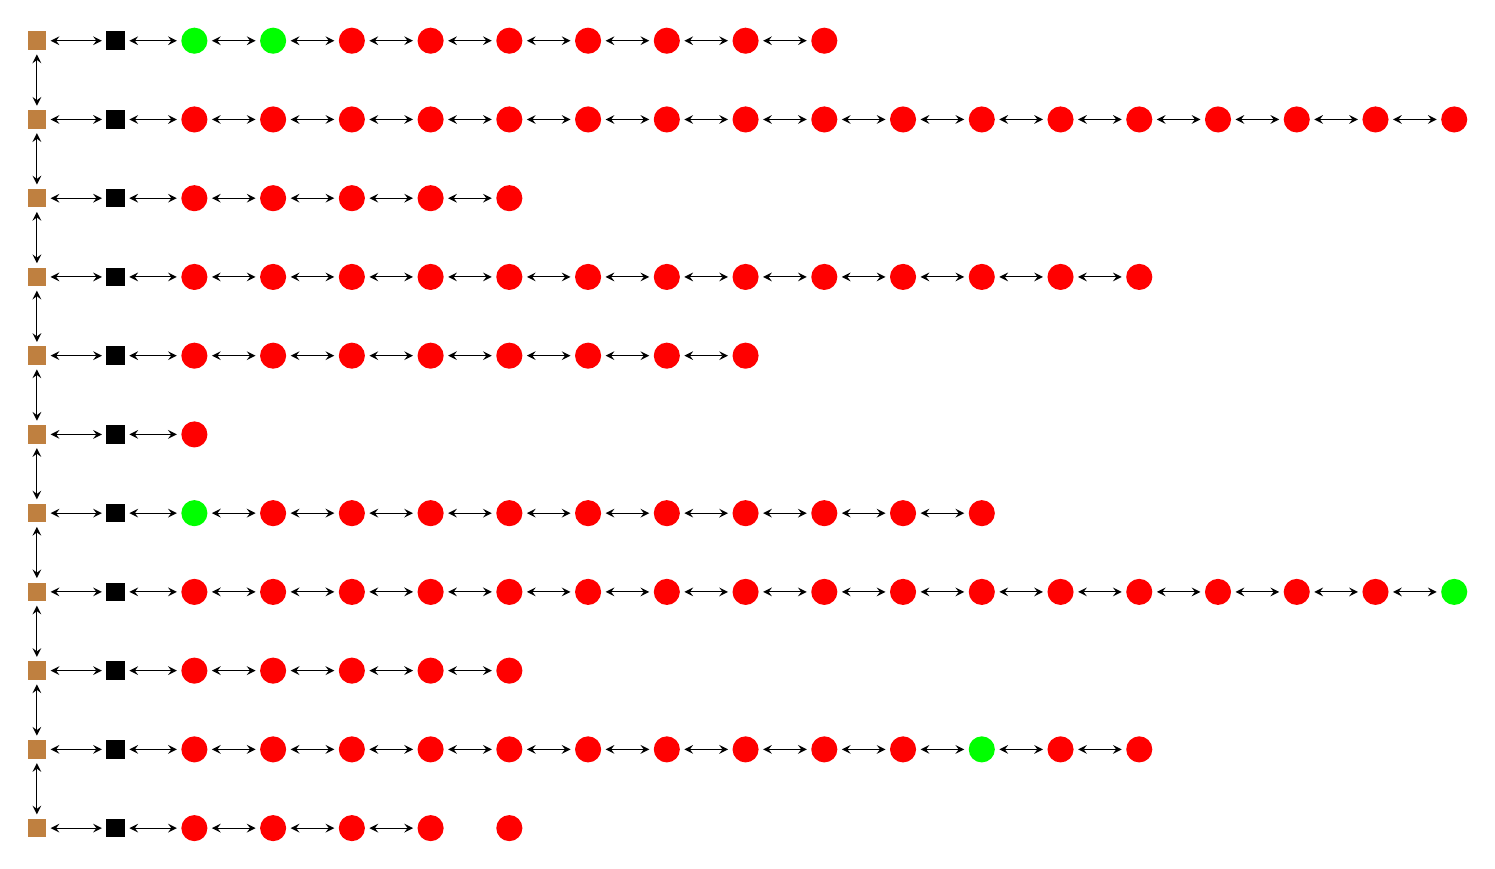
\begin{tikzpicture}[rotate=270,font=\tiny,
   oc/.style={fill=black,rectangle,minimum size=0.01cm,font=\tiny},
     feeder/.style={fill=brown,rectangle,minimum size=0.005cm,font=\tiny},
   Producer/.style={fill=green,circle,minimum size=0.01cm},
     Consumer/.style={fill=red,circle,minimum size=0.01cm},
   Connection/.style={<->, >=stealth, shorten <=0.05cm, shorten >=0.05cm}]
 \draw node[oc] (oc1) at (-5,0){};
 \draw node[oc] (oc2) at (-4,0){};
 \draw node[oc] (oc3) at (-3,0){};
 \draw node[oc] (oc4)  at (-2,0){};
 \draw node[oc](oc5)  at (-1,0){};
 \draw node[oc] (oc6)  at (0,0){};
 \draw node[oc] (oc7) at (1,0){};
 \draw node[oc] (oc8)  at (2,0){};
 \draw node[oc] (oc9) at (3,0){};
 \draw node[oc] (oc10) at (4,0){};
 \draw node[oc] (oc11) at (5,0){};

 \draw node[feeder] (feeder1) at (-5,-1){};
 \draw node[feeder] (feeder2) at (-4,-1){};
 \draw node[feeder] (feeder3) at (-3,-1){};
 \draw node[feeder] (feeder4)  at (-2,-1){};
 \draw node[feeder](feeder5)  at (-1,-1){};
 \draw node[feeder] (feeder6)  at (0,-1){};
 \draw node[feeder] (feeder7) at (1,-1){};
 \draw node[feeder] (feeder8)  at (2,-1){};
 \draw node[feeder] (feeder9) at (3,-1){};
 \draw node[feeder] (feeder10) at (4,-1){};
 \draw node[feeder] (feeder11) at (5,-1){};

 \draw [Connection] (feeder1) to (feeder2);
 \draw [Connection] (feeder2) to (feeder3);
 \draw [Connection] (feeder3) to (feeder4);
 \draw [Connection] (feeder4) to (feeder5);
 \draw [Connection] (feeder5) to (feeder6);
 \draw [Connection] (feeder6) to (feeder7);
 \draw [Connection] (feeder7) to (feeder8);
 \draw [Connection] (feeder8) to (feeder9);
 \draw [Connection] (feeder9) to (feeder10);
 \draw [Connection] (feeder10) to (feeder11);

\draw [Connection] (feeder1) to (oc1);
\draw [Connection] (feeder2) to (oc2);
\draw [Connection] (feeder3) to (oc3);
\draw [Connection] (feeder4) to (oc4);
\draw [Connection] (feeder5) to (oc5);
\draw [Connection] (feeder6) to (oc6);
\draw [Connection] (feeder7) to (oc7);
\draw [Connection] (feeder8) to (oc8);
\draw [Connection] (feeder9) to (oc9);
\draw [Connection] (feeder10) to (oc10);
\draw [Connection] (feeder11) to (oc11);


 \foreach \pos in {1,2} {
   \node [Producer] (p10\pos)at (-5,\pos) {};
 }

 \foreach \pos in {3,4,5,6,7,8,9} {
   \node [Consumer] (c10\pos)at (-5,\pos) {};
 }

 \foreach \pos in {1,2,3,4,5,6,7,8,9,10,11,12,13,14,15,16,17} {
   \node [Consumer] (c20\pos)at (-4,\pos) {};
 }

 \foreach \pos in {1,2,3,4,5} {
   \node [Consumer] (c30\pos)at (-3,\pos) {};
 }


 \foreach \pos in {1,2,3,4,5,6,7,8,9,10,11,12,13} {
   \node [Consumer] (c40\pos)at (-2,\pos) {};
 }


 \foreach \pos in {1,2,3,4,5,6,7,8} {
   \node [Consumer] (c50\pos)at (-1,\pos) {};
 }


 \foreach \pos in {1} {
   \node [Consumer] (c60\pos)at (0,\pos) {};
 }


 \foreach \pos in {1} {
   \node [Producer] (p70\pos)at (1,\pos) {};
 }


 \foreach \pos in {2,3,4,5,6,7,8,9,10,11} {
   \node [Consumer] (c70\pos)at (1,\pos) {};
 }


 \foreach \pos in {17} {
   \node [Producer] (p80\pos)at (2,\pos) {};
 }

 \foreach \pos in {1,2,3,4,5,6,7,8,9,10,11,12,13,14,15,16} {
   \node [Consumer] (c80\pos)at (2,\pos) {};
 }

 \foreach \pos in {1,2,3,4,5} {
   \node [Consumer] (c90\pos)at (3,\pos) {};
 }

 \foreach \pos in {11} {
   \node [Producer] (p100\pos)at (4,\pos) {};
 }

 \foreach \pos in {1,2,3,4,5,6,7,8,9,10,12,13} {
   \node [Consumer] (c100\pos)at (4,\pos) {};
 }

 \foreach \pos in {1,2,3,4,5} {
   \node [Consumer] (c110\pos)at (5,\pos) {};
 }


 \draw [Connection] (oc1) to (p101);
 \draw [Connection] (p101) to (p102);
 \draw [Connection] (p102) to (c103);
 \draw [Connection] (c103) to (c104);
 \draw [Connection] (c104) to (c105);
 \draw [Connection] (c105) to (c106);
 \draw [Connection] (c106) to (c107);
 \draw [Connection] (c107) to (c108);
 \draw [Connection] (c108) to (c109);
 
\draw [Connection] (oc2) to (c201);
\draw [Connection] (c201) to (c202);
\draw [Connection] (c202) to (c203);
\draw [Connection] (c203) to (c204);
\draw [Connection] (c204) to (c205);
\draw [Connection] (c205) to (c206);
\draw [Connection] (c206) to (c207);
\draw [Connection] (c207) to (c208);
\draw [Connection] (c208) to (c209);
\draw [Connection] (c209) to (c2010);
\draw [Connection] (c2010) to (c2011);
\draw [Connection] (c2011) to (c2012);
\draw [Connection] (c2012) to (c2013);
\draw [Connection] (c2013) to (c2014);
\draw [Connection] (c2014) to (c2015);
\draw [Connection] (c2015) to (c2016);
\draw [Connection] (c2016) to (c2017);

\draw [Connection] (oc3) to (c301);
\draw [Connection] (c301) to (c302);
\draw [Connection] (c302) to (c303);
\draw [Connection] (c303) to (c304);
\draw [Connection] (c304) to (c305);

\draw [Connection] (oc4) to (c401);
\draw [Connection] (c401) to (c402);
\draw [Connection] (c402) to (c403);
\draw [Connection] (c403) to (c404);
\draw [Connection] (c404) to (c405);
\draw [Connection] (c405) to (c406);
\draw [Connection] (c406) to (c407);
\draw [Connection] (c407) to (c408);
\draw [Connection] (c408) to (c409);
\draw [Connection] (c409) to (c4010);
\draw [Connection] (c4010) to (c4011);
\draw [Connection] (c4011) to (c4012);
\draw [Connection] (c4012) to (c4013);

\draw [Connection] (oc5) to (c501);
\draw [Connection] (c501) to (c502);
\draw [Connection] (c502) to (c503);
\draw [Connection] (c503) to (c504);
\draw [Connection] (c504) to (c505);
\draw [Connection] (c505) to (c506);
\draw [Connection] (c506) to (c507);
\draw [Connection] (c507) to (c508);

\draw [Connection] (oc6) to (c601);

\draw [Connection] (oc7) to (p701);
\draw [Connection] (p701) to (c702);
\draw [Connection] (c702) to (c703);
\draw [Connection] (c703) to (c704);
\draw [Connection] (c704) to (c705);
\draw [Connection] (c705) to (c706);
\draw [Connection] (c706) to (c707);
\draw [Connection] (c707) to (c708);
\draw [Connection] (c708) to (c709);
\draw [Connection] (c709) to (c7010);
\draw [Connection] (c7010) to (c7011);

\draw [Connection] (oc8) to (c801);
\draw [Connection] (c801) to (c802);
\draw [Connection] (c802) to (c803);
\draw [Connection] (c803) to (c804);
\draw [Connection] (c804) to (c805);
\draw [Connection] (c805) to (c806);
\draw [Connection] (c806) to (c807);
\draw [Connection] (c807) to (c808);
\draw [Connection] (c808) to (c809);
\draw [Connection] (c809) to (c8010);
\draw [Connection] (c8010) to (c8011);
\draw [Connection] (c8011) to (c8012);
\draw [Connection] (c8012) to (c8013);
\draw [Connection] (c8013) to (c8014);
\draw [Connection] (c8014) to (c8015);
\draw [Connection] (c8015) to (c8016);
\draw [Connection] (c8016) to (p8017);

\draw [Connection] (oc9) to (c901);
\draw [Connection] (c901) to (c902);
\draw [Connection] (c902) to (c903);
\draw [Connection] (c903) to (c904);
\draw [Connection] (c904) to (c905);

\draw [Connection] (oc10) to (c1001);
\draw [Connection] (c1001) to (c1002);
\draw [Connection] (c1002) to (c1003);
\draw [Connection] (c1003) to (c1004);
\draw [Connection] (c1004) to (c1005);
\draw [Connection] (c1005) to (c1006);
\draw [Connection] (c1006) to (c1007);
\draw [Connection] (c1007) to (c1008);
\draw [Connection] (c1008) to (c1009);
\draw [Connection] (c1009) to (c10010);
\draw [Connection] (c10010) to (p10011);
\draw [Connection] (p10011) to (c10012);
\draw [Connection] (c10012) to (c10013);


\draw [Connection] (oc11) to (c1101);
\draw [Connection] (c1101) to (c1102);
\draw [Connection] (c1102) to (c1103);
\draw [Connection] (c1103) to (c1104);

 \end{tikzpicture}
 }
 \caption{Feeder diagram. Brown nodes are feeder junctions, numbered 1 to 11 from top to bottom.  Black nodes are the overcurrent relays, which ensure that the total power flowing in and out of the feeder is below 20 kW. The green nodes are the junction points for the producers ($5$), and the red nodes are junction points for the consumers ($97$). There are $102$ prosumers in total.}
 \label{fig:feeder}
 \end{figure}


\begin{figure}[t]
\centering
\begin{tikzpicture}
\begin{axis}[
  font=\footnotesize,
  width=\columnwidth,
  height=0.61\columnwidth,
  ymin=-1,
 legend columns=3, 
  legend style={font=\fontsize{5}{6}\selectfont,cells={align=left},text width=4.3em,text height=1.5ex,text depth=.5ex,row sep=0.1em},
  ymax=220,
grid=both,
    grid style={line width=.1pt, draw=gray!10},
    major grid style={line width=.2pt,draw=gray!50},
  xmin=-1,
  xmax=97,
  legend pos=north west,
  xlabel=Time,
  ylabel={[kWh]},
  ytick={0, 50, 100, 150, 200},
  xtick={0, 16, 32, 48, 64, 80, 95},
  xticklabels={0:00, 4:00, 8:00, 12:00, 16:00,  20:00, 23:45},
]
\addplot[no markers, solid, greenline, semithick] table[x expr=\coordindex, y=WithoutBattery,  comment chars={\%}, col sep=comma] {diagrams/interval-energy-traded.csv};
\addlegendentry{Total energy traded (Test A)};
\addplot[no markers, solid, blackLine, semithick] table[x expr=\coordindex, y=WithBattery5,  comment chars={\%}, col sep=comma] {diagrams/interval-energy-traded.csv};
\addlegendentry{Total energy traded (Test C)};
\addplot[no markers, solid, goldLine, semithick] table[x expr=\coordindex, y=WithBattery12,  comment chars={\%}, col sep=comma] {diagrams/interval-energy-traded.csv};
\addlegendentry{Total energy traded (Test D)};
\addplot[no markers, solid, blueLine, semithick] table[x expr=\coordindex, y=TotalProduction, comment chars={\%}] {diagrams/TotalProductionConsumption.csv};
\addlegendentry{Total production};
\addplot[no markers, solid, redLine, semithick] table[x expr=\coordindex, y=TotalConsumption, comment chars={\%}] {diagrams/TotalProductionConsumption.csv};
\addlegendentry{Total consumption};
\end{axis}
\end{tikzpicture}
\caption{Load profile (i.e., total consumption) and generation profile (i.e., total production) in kWh per 15 minute interval aggregated across the microgrid.  The graph also shows the energy traded per interval without battery, with battery and prediction window of 5 intervals, and with battery and prediction window of 12 intervals. Note that the amount of energy traded can be lower than both demand and supply at the same time because of safety constraints, which limit the amount of energy that can flow out of the producers' feeders.}
\label{fig:profile}
% \vspace{-0.2in}
\end{figure}



\begin{figure}[ht]
\begin{tikzpicture}
\begin{axis}[
  font=\footnotesize,
  width=0.94\columnwidth,
  height=0.65\columnwidth,
  ymin=-0.2,
  ymax=10,
  xmin=28,
  xmax=95,
  ylabel={Energy [kWh]},
  xtick={0, 16, 32, 48, 64, 80, 95},
  xticklabels={0:00, 4:00, 8:00, 12:00, 16:00,  20:00, 23:45},
grid=both,
    grid style={line width=.1pt, draw=gray!10},
    major grid style={line width=.2pt,draw=gray!50},
]
\addplot[mark=*, mark size=0.5, solid, blueLine, semithick] table[x= startTime, y=Energy, comment chars={\%}] {diagrams/outputTestA.csv};
\end{axis}
\begin{axis}[
  font=\footnotesize,
  width=0.94\columnwidth,
  height=0.65\columnwidth,
  ymin=-1,
  ymax=50,
  xmin=28,
  xmax=95,
  xtick={},
  xticklabels={},
  ylabel={Offer length [intervals]},
  ytick={0, 10, 20, 30, 40, 50},
  axis y line*=right,
  legend pos=north east,
]
\addlegendimage{blueLine, semithick}
\addlegendentry{Energy}
\addplot[ybar interval,redLine] table[ x=startTime,y=Availability, comment chars={\%}] {diagrams/outputTestA.csv};
\addlegendentry{Offer length}
\end{axis}
\end{tikzpicture}
\caption{Energy offered in each time interval by the first prosumer of the first feeder when using a battery (blue line). The red bars indicate the number of contiguous intervals for which the offer is valid. The total battery capacity is 90 kWh. It is assumed that the battery charges at a rate of 10 kWh per interval. Producers are assumed to keep the battery available till the end of the test, which is the 95th interval. Consequently, the red bars taper off in consecutive intervals.}
\label{fig:batteryEffect}
\end{figure}

 
 \begin{figure}[ht]
	\centering		\includegraphics[width=1\columnwidth]{diagrams/testbed.jpg}
	\caption{Hardware test bed.}
   \label{fig:testbed_architecture}
\end{figure}


\begin{table}[ht]    
%\setlength{\tabcolsep}{4pt}
\caption{Parameter Values for Experiments (See Table \ref{tab:symbols})}
\label{table:test-parameters}  
\centering
\begin{tabular}{lllll}
& A  & B  & C  & D     \\ \cline{2-5} 
\multicolumn{1}{l|}{$\Delta$[m]}   & 15 & 15 & 15 & 15   \\
\multicolumn{1}{l|}{$\Delta_s$ [s]}   & 5 & 5 & 5 & 5   \\
\multicolumn{1}{l|}{$\hat{\Delta}$ [s]} & 120 & 120 & 120 & 120   \\
\multicolumn{1}{l|}{$L$}          & 2,3,5,7,10,13  & 2,3,7,10  & 5  & 13    \\
\multicolumn{1}{l|}{Battery}     & no & yes & yes & yes \\
\hline
\multicolumn{1}{l|}{Figure}     & \ref{fig:multihorizon} &\ref{fig:multihorizon} & \ref{fig:allocate1NRG},\ref{fig:time},\ref{fig:profile},\ref{fig:multihorizon} &  \ref{fig:profile},\ref{fig:multihorizon} 
\end{tabular}
\end{table}

  In this example, a prosumer is modeled as an actor with an energy generation and consumption profile for the near future. In practice, the generation profile would be typically derived from predictions based on the weather, energy generation capabilities, and the amount of battery storage available. The consumption profile would be derived from flexible power loads, like  washers and electric vehicles.  

To represent future generation or consumption at a certain time, % loads as offers to the platform the 
resource types encode %composing an offer would simply be the
timestamps for 15-minute intervals, during which the power will be generated or consumed. 
As an example, consider a battery that has 500 Wh energy, which could be discharged any time between 9AM and 10AM.
%A simplified example (using clock time, rather than epoch time) could be a batter has stored 500W-h of energy and makes it available from 9:00-10:00AM. 
This can be represented by an offer having resource types 900, 915, 930, and 945, specifying a quantity of 500 Wh for each.

 
 For our simulation, the prosumer energy profiles are load traces recorded by Siemens during a day from a microgrid in Germany, containing $102$ homes %across $11$ feeders 
 ($5$ producers and $97$ consumers). Since the dataset does not include prices, we assume reservation prices to be uniform in our experiments, and focus on studying the amount of energy traded and the performance of the system. %Table \ref{tab:prosumers}
%Figure~\ref{fig:feeder} describes the feeder structure, the number of participants per feeder, and  the feeder safety limits.

%Each trace was divided into 15-minute time intervals that the prosumer can sumbit as an offer.

Figure~\ref{fig:totals} shows the total production (green) and consumption (red) across this microgrid, as well as the total energy traded per interval (blue) using our platform. The horizontal axis shows the starting time for each of the $96$ intervals.


\ifExtended
In this implementation, the prosumers do not submit all of the offers simultaneously, instead they post offers for the 5 intervals beyond the current interval being finalized. The justification for this is that a prosumer may not know their energy profile for the entire day and may only be able to make accurate estimates for a few future intervals at a time. Similarly a solver may be implemented to create matches for only the interval being finalized or may ``look-ahead'' at future offers and create match that may not be optimal for the current interval but allows better matches to be made in the future. This is a trade off between the complexity of the problem and how close the solution is to the global optimum.
%In this implementation, our solver finds a match for the current interval while looking ahead at the next 4 intervals.
%This can be seen in Figure  \ref{fig:MultipleSolutions},
%Since additional offers are being submitted during the simulation 
\Aron{This will be very unclear to the reviewers since the platform described in this paper does not do this.}
\Scott{Is that a better explanation?}
% Since the prosumers have a schedule for their energy consumption, they can post offers for several intervals in the future. By including offers for multiple intervals, the solver can find assignments for future intervals.
% As more information becomes available over time, the solver may find better solutions, as shown by Figure \ref{fig:MultipleSolutions}.
\fi

\ifExtended
For example, in the first interval, the green solution is submitted, which includes a matching for then current interval (at 7:30AM) as well as the next four intervals.
%, 7:45, 8:00, 8:15, and 8:30. 
Then, in the second interval, the yellow solution is added, which supersedes the green solution for intervals at 8:00AM, 8:15AM, and 8:30AM because more offers are now available and a better solution may be found. %, it also adds a solution for the 8:45 interval. 
% In this simulation, the solver solves for the current interval to be finalized as well as the next 4 intervals. The number of additional intervals can be varied to trade off between solve time, and overall solution optimality. 
\fi

%The solver time in this casestudy was 3s on average. Compared to carpool problem, this problem has more variables

\ifExtended
Figure \ref{fig:solve-time} shows the running time of the solver.
%with the 4 interval look-ahead. 
The time on the horizontal axis is the actual clock time, which shows that the simulation ran for about an hour. We also note that at about 20 minutes from the beginning (i.e., around interval 48), %which corresponds to noon in the simulated time series, 
solving time begins to increase. 
This increase is due to offers being made that span multiple intervals, i.e there are multiple resource types as in our 500Wh example.
\fi
%These kind of offers are possible because some of the selling offers can be valid for a range of future intervals instead of requiring immediate consumption (thanks to battery storage). 
%\Aron{Again, the reviewer will have no idea what we are talking about here.}
%\Scott{Is that more clear?}

In another simulation, we exercise the hybrid solver architecture by running multiple solvers, and after some time, cause one to fail. This result is shown in Figure~\ref{fig:failure}. The narrow vertical red line indicates when solver 1 fails at 8:15AM. Up until that point, solver 1 submitted the green, yellow, light blue, orange solutions, with the final solution being red.% Since the solver computes matching for the subsequent four intervals.
%solver 1 has a solution for them but they are not improved as new information is available. 
On the other hand we see that solver 2 continues to provide solutions for later intervals. 

% %To evaluate the performance of our solution, we take the following measurements:  running time of the solver to find a potential solution; time taken by the smart contract to finalize an interval\Aron{What is included in this? How is it measured? Very uncler!};  percentage of demand that is met with trades;  percentage of supply that is consumed through trades. 

% Results are shown in Figure \ref{fig:totals}.
% \Aron{?}

% \Aron{Font in figure is unreadable, it needs to be orders of magnitude bigger.}
% Figure \ref{fig:finalize-time} shows the time between the finalize event and the finalization of trades.

%The vertical narrow red line identifies the interval at 9:00am. In Solution 1 (), the purple bars were the last solution provided by Solver 1, while Solver 2 provides 4 more solutions during the next 4 intervals. 






%\Aron{We should move the detailed descriptions from the figure captions into the main text!}
 